% Figure 4: Lens-type transfer model
% Three lens types plotted on Generativity x Format-Dependency axes.
% Circle radius proportional to |A5->A6 gap|.

\usepackage{tikz}
\usetikzlibrary{positioning,arrows.meta,shapes.geometric,calc}

\begin{figure}[t]
\centering
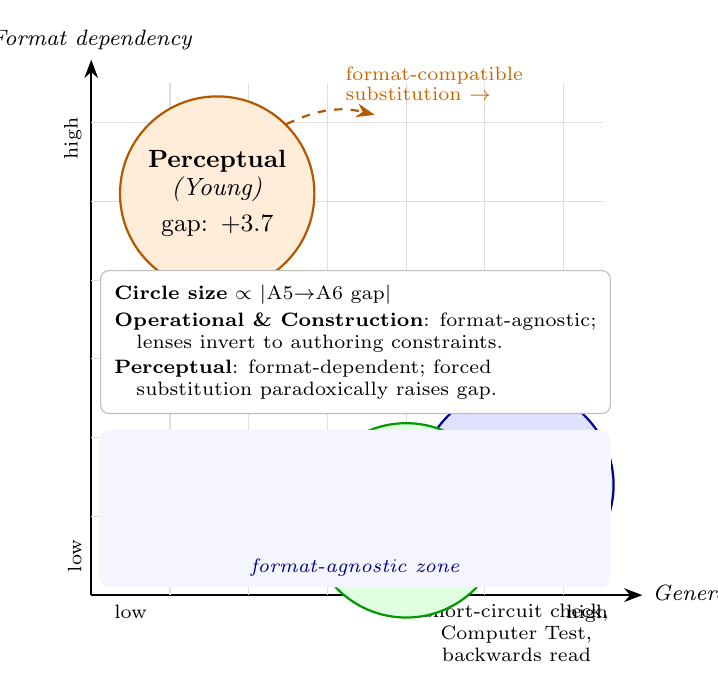
\begin{tikzpicture}[
  font=\small,
  >=Stealth,
  % Shared circle style; radius set per node via minimum size
  lens/.style={
    draw, circle, align=center, text width=2.0cm,
    inner sep=2pt, line width=0.8pt
  },
  operational/.style={lens, fill=blue!12,  draw=blue!60!black},
  construct/.style= {lens, fill=green!12, draw=green!60!black},
  perceptual/.style={lens, fill=orange!15, draw=orange!70!black},
  axislabel/.style={font=\footnotesize\itshape},
  sublabel/.style={font=\scriptsize, align=center},
]

% ---------------------------------------------------------------
% Coordinate system: x = Generativity (0..6), y = Format-dep (0..6)
% ---------------------------------------------------------------

% Invisible bounding frame to fix canvas size
\draw[white, use as bounding box] (-0.8,-0.9) rectangle (7.6,7.2);

% --- Axes ---
\draw[->, thick] (0,0) -- (7.0,0)
  node[right, axislabel] {Generativity};
\draw[->, thick] (0,0) -- (0,6.8)
  node[above, axislabel] {Format dependency};

% Tick labels on x-axis
\node[below, font=\scriptsize] at (0.5,0) {low};
\node[below, font=\scriptsize] at (6.3,0) {high};

% Tick labels on y-axis
\node[left, font=\scriptsize, rotate=90, anchor=south] at (0,0.5)  {low};
\node[left, font=\scriptsize, rotate=90, anchor=south] at (0,5.8)  {high};

% Light grid
\foreach \x in {1,2,3,4,5,6}
  \draw[gray!25, thin] (\x,0) -- (\x,6.5);
\foreach \y in {1,2,3,4,5,6}
  \draw[gray!25, thin] (0,\y) -- (6.5,\y);

% ---------------------------------------------------------------
% OPERATIONAL (Katz): HIGH generativity, LOW format dependency
%   Position: x=5.4, y=1.4
%   |gap| = 1.6  => minimum size = 1.6 * 10 + 14 = 30pt  (scaled)
% ---------------------------------------------------------------
\node[operational, minimum size=44pt] (op) at (5.4, 1.4) {
  \textbf{Operational}\\[-1pt]
  \textit{(Katz)}\\[2pt]
  gap: $+1.6$
};
\node[sublabel, below=4pt of op] {
  short-circuit check,\\
  Computer Test,\\
  backwards read
};

% ---------------------------------------------------------------
% CONSTRUCTION (Snyder): MEDIUM-HIGH generativity, LOW format dep
%   Position: x=4.0, y=1.0
%   |gap| = 0.7  => minimum size smallest
% ---------------------------------------------------------------
\node[construct, minimum size=32pt] (con) at (4.0, 0.95) {
  \textbf{Construction}\\[-1pt]
  \textit{(Snyder)}\\[2pt]
  gap: $-0.7$
};
\node[sublabel, above=4pt of con] {
  load-bearing test,\\
  solve-path uniqueness
};

% ---------------------------------------------------------------
% PERCEPTUAL (Young): LOW generativity, HIGH format dependency
%   Position: x=1.4, y=5.2
%   |gap| = 3.7  => minimum size largest
% ---------------------------------------------------------------
\node[perceptual, minimum size=60pt] (per) at (1.6, 5.1) {
  \textbf{Perceptual}\\[-1pt]
  \textit{(Young)}\\[2pt]
  gap: $+3.7$
};
\node[sublabel, below=4pt of per] {
  visual grammar,\\
  layout hierarchy,\\
  visual resolution
};

% ---------------------------------------------------------------
% Paradox arrow: Perceptual -> upper-right quadrant
% Represents: forced substitution drives quality up
% ---------------------------------------------------------------
\draw[->, dashed, thick, orange!70!black, bend left=20]
  (per.north east)
  to node[midway, above right, align=left, font=\scriptsize,
          text=orange!80!black, xshift=2pt] {
    format-compatible\\[-1pt]
    substitution $\to$
  }
  (3.6, 6.1);

% ---------------------------------------------------------------
% Diagonal shading annotation band
% "format-agnostic zone" along bottom
% ---------------------------------------------------------------
\fill[blue!4, rounded corners=4pt]
  (0.1, 0.1) rectangle (6.6, 2.1);
\node[font=\scriptsize\itshape, text=blue!50!black, align=center]
  at (3.35, 0.35) {format-agnostic zone};

% ---------------------------------------------------------------
% Key annotation box (bottom-right)
% ---------------------------------------------------------------
\node[draw=gray!50, fill=white, rounded corners=3pt,
      align=left, font=\scriptsize, inner sep=5pt,
      anchor=south east] at (6.6, 2.3) {
  \textbf{Circle size} $\propto$ $|$A5$\to$A6 gap$|$\\[2pt]
  \textbf{Operational \& Construction}: format-agnostic;\\
  \quad lenses invert to authoring constraints.\\[1pt]
  \textbf{Perceptual}: format-dependent; forced\\
  \quad substitution paradoxically raises gap.
};

\end{tikzpicture}

\caption{The lens-type transfer model. \textbf{Operational} lenses (Katz) invert
directly to authoring constraints and are format-agnostic---named tests such as the
Computer Test or backwards-read check become authoring rules with minimal adaptation.
\textbf{Construction} lenses (Snyder) are already authoring-compatible; the
A5/A6 distinction largely collapses, producing a small negative gap ($-0.7$).
\textbf{Perceptual} lenses (Young) require specific output material (layout,
visual hierarchy) and produce the largest A5$\to$A6 gap---positive in this study
because the text-only format forced a domain-native substitute for visual instincts,
yielding higher-quality output when adaptation succeeded (dashed arrow).}
\label{fig:lens}
\end{figure}
